\chapter{Black hole at the Galactic center? (stellar orbits)}

%TODO replace homework with actually doable and physical arguments
%TODO restructure lab to make sense, be clear, organized
%TODO make equal-area section length^2, not arcsec^2

\section{``Observing'' Black Holes}

Black Holes are robustly predicted by Einstein's theory of General Relativity, the current state-of-
the-art in mathematical explanations of gravitational phenomenon. It has also been demonstrated
theoretically that such extreme objects naturally arise in the late-stages of stellar evolution for the
most massive stars. However, they are difficult to observe for a simple reason: by their very nature (as
suggested by their name), they do not emit light. Nonetheless, their presence can be inferred indirectly
through their gravitational effect on other objects. Astronomers and physicists have discovered so many
independent and corroborating lines of evidence of this type detected that the existence of black holes
is now considered a well-established scientific fact.

The detection of gravitational waves by the Laser Interferometer Gravitational-Wave Observatory
(LIGO) in 2017 is arguably the most stunning and conclusive evidence of this to date. In a
beautiful demonstration of the validity of General Relativity, the perturbations in space and time
(Gravitational Waves) characteristically generated by the coalescence of a binary black hole pair were
detected on Earth after having traveled at the speed of light from their source roughly one billion light
years away. The clarity of this signal and its agreement with predictions have all but conclusively
determined the existence of black holes.

However, less direct (but nonetheless extremely convincing) evidence for the existence of black holes
had been well known in observational astronomy for some time. In this lab, you will explore one of the
most striking examples of these observational signatures: the orbits of stars around Sag A*, the radio source that is collocated with the `dark attractor' at the center of our galaxy that is almost certainly a Super-Massive Black Hole (SMBH). Astronomers now know that almost all galaxies have such behemoths at their centers, and that they likely play a fundamental role in galaxy evolution. The discovery of one at the center of the Milky Way (roughly 8 kpc distant) was an important step in the development of this SMBH paradigm. In this lab, you will partially reproduce a simplified version of the analysis that led astronomers to this exciting conclusion.

\textbf{Rubric Rows to be assessed:} C4 and C5 (for Kepler's 2nd Law); D8, D9, and G1 (for Kepler's 3rd Law mass estimation); F1 and F2 (for all parts)

\section{Newtonian Dynamics and Orbital Dynamics Basics}

The trajectories of objects moving under the influence of gravity are generally called \textit{orbits}. Newton's
Law of Gravity, while not an adequate description for extreme gravitational fields, is nonetheless a good
approximation generally and in the specific cases of orbits we'll be examining. It is given by
\begin{equation}\label{gc:eq:newton}
 F_\textrm{grav} = G \frac{m_1 \: m_2}{r^2} \, ,
\end{equation}
where $F_\textrm{grav}$ is the force of gravity between any two objects of mass $m_1$ and $m_2$ a distance $r$ from each other. $G$ is Newton's Gravitational Constant, whose value in CGS (Centimeters Grams Seconds) units
is $6.67 \times 10^{-8}\:\textrm{cm}^3 \: \textrm{g}^{-1} \: \textrm{s}^{-2}$. The gravitational force is attractive: it pulls objects together. This, coupled
with Newton's Second Law of Motion relating the force acted upon an object $F$ and its acceleration $a$,
\begin{equation}
 F = ma \,,
\end{equation}
tells us that \textit{the acceleration of an object due to gravity will be greater in stronger gravitational fields}.
These two fundamental physical laws can be used to derive the properties of Newtonian gravitational
orbital motion. We won't do so here, but instead just cover some of the key implications, concisely
stated by Kepler's Laws of Orbital Motion. These Laws, which are concise mathematical descriptions
of how the planets move in the Solar System, preceded Newton's work by nearly a century, and were
based solely on observational data. Newton's work on gravity and motion explained, at a deeper level,
why Kepler's Laws are as they are.

\subsection{Kepler's Laws}

\subsubsection{Kepler's First Law}

Kepler’s First Law states that \textbf{A planet orbits the Sun in an ellipse, with the Sun at one focus
of the ellipse.} This is true generally for any mass orbiting a much more massive object. An \textit{ellipse} is a
generalization of a circle, allowing for the circle to be stretched along a certain direction. See Figure~\ref{gc:fig:ellipse} for details.

\begin{figure}
	\centering
	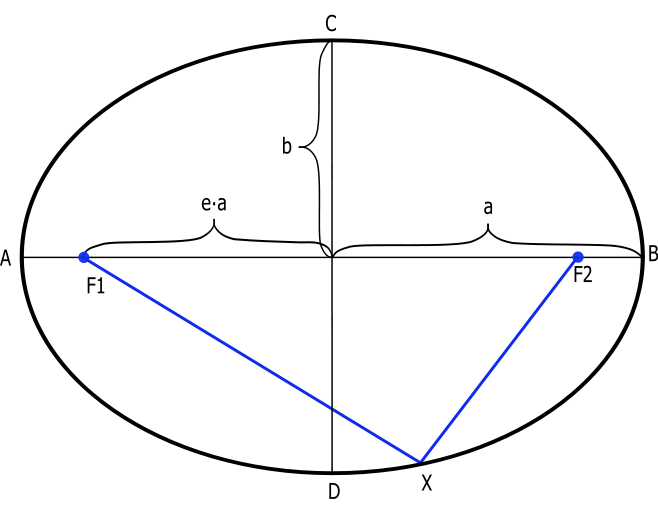
\includegraphics[width=0.6\textwidth]{galactic-center/ellipse.png}
	\caption{The geometry of an ellipse: $a$ is the semi-major axis of the ellipse, F1 and F2 are each a
		focus of the ellipse, $b$ is the semi-minor axis, and $e$ is the eccentricity. The eccentricity describes
		the extent to which the ellipse is oblong: an ellipse with $e = 0$ is just a circle. The foci are defined such
		that the distance from F1 to X, added to the distance from F2 to X, is the same no matter where X
		is located on the ellipse. For a circle, the foci coincide at the center. The Newtonian generalization of
		Kepler's First Law tells us that a small mass will orbit a much larger mass on an ellipse, and the larger
		mass will be located at one of the foci.}\label{gc:fig:ellipse}
\end{figure}

\subsubsection{Kepler's Second Law}

The second law states that \textbf{a line connecting a planet to the Sun sweeps out equal areas in
equal time intervals}. This concept is demonstrated in Figure~\ref{gc:fig:keplers-2nd-ellipse}. As a consequence of this, when a
planet is closer to the sun, it orbits with a faster velocity. Furthermore, planets that have more circular
orbits will have more uniform velocities over the course of their orbit than those with very eccentric
orbits.

\begin{figure}
	\centering
	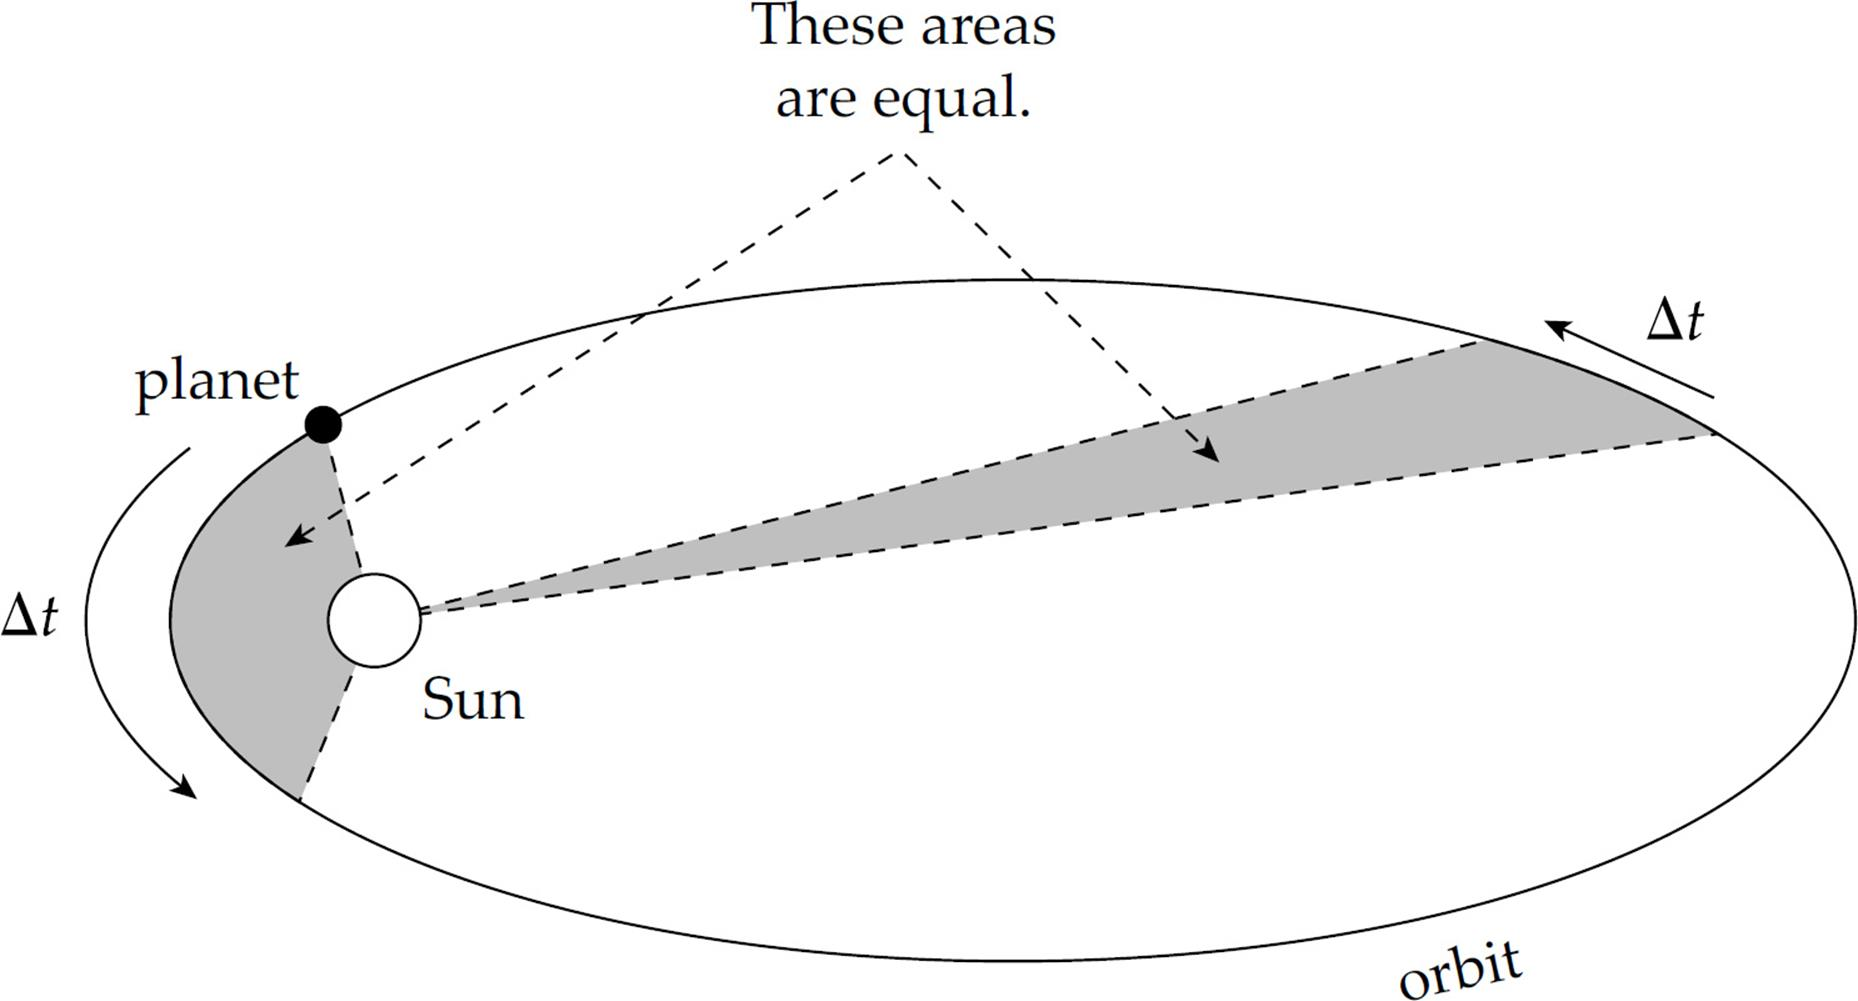
\includegraphics[width=0.7\textwidth]{galactic-center/keplers-2nd-ellipse.png}
	\caption{Illustration of Kepler’s Second Law. The shaded regions are of equal area, so by Kepler’s Second Law, the
		planet passes through each region of the orbit in the same amount of time. Since the region of the orbit
		where the planet is closest to the Sun is a much further distance, and speed is change in position over
		change in time, the planet will move with a much faster average speed than at the other portion of the
		orbit, far away from the sun.}\label{gc:fig:keplers-2nd-ellipse}
\end{figure}

\subsubsection{Kepler's Third Law}

Kepler’s Third law addresses the path of an object $m$ as it orbits a much more massive object of mass $M$. Specifically, it relates the orbital period $P$ (the time it takes for one complete orbit to occur) to the semi-major axis $a$ of the ellipse according to
\begin{equation}\label{gc:eq:kepler-3}
 P^2 = \frac{4 \pi^2}{G M} a^3 \,,
\end{equation}
where other objects are also considered to be not affecting the orbit of $m$. \textbf{This is the
	equation you will be using in the central calculation of the lab.}

An important qualification to be made about Kepler’s Laws is that they apply only to two-body
systems. Kepler’s Third law breaks down when you have more than 2 orbiting objects in a system.
However, they are nonetheless a very good approximation for the orbits of small masses around a much
larger mass, in which case the gravitational force of the massive object dominates over the intra-small-
object interactions, and thus each smaller body approximately behaves independently from the other
small objects. And so the motion of each small object, to a good approximation, can be modeled by
Kepler’s Laws.

\subsection{Escape speed}

Another important concept in orbital dynamics --- which comes from the general Newtonian understanding of orbits --- is that of the escape speed. This is the minimum speed that an object must reach
to break out of its orbit at a certain radius from the central massive object. The escape speed $v_\textrm{escape}$ at a
distance $r$ from the center of a mass $M$ is given by
\begin{equation}\label{gc:eq:escape-speed}
 v_\textrm{escape} = \sqrt{\frac{2 G M}{r}} \,.
\end{equation}
An orbiting object that achieves a speed greater than this is unbound to the object it is orbiting, and will escape its gravitational pull, flying out of the system entirely.

\section{General Relativity}

Despite the great success of Newtonian dynamics in explaining a wide variety of the celestial motions
that we observe, this picture of gravity is incomplete and inaccurate in the most extreme regimes,
where General Relativity is required. A fully self-consistent description of relativity is well beyond the
scope of these notes (or this course), but the fundamental conceptual premise is easily stated: gravity
is not a magical “attraction at a distance” between objects with mass, but rather the result of curved
space-time, which is an effect of all mass. A helpful analogy is that of a sheet of fabric being depressed
by a massive object (see Figure~\ref{gc:fig:gen-rel-sheet}). Other objects placed on this depressed fabric will begin orbiting
around the massive object.

\begin{figure}
	\centering
	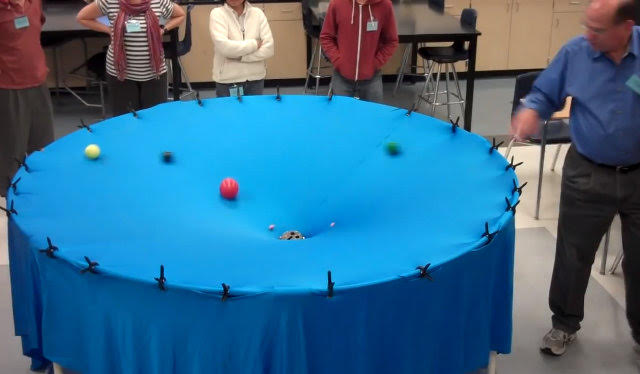
\includegraphics[width=\textwidth]{galactic-center/gen-rel-sheet.png}
	\caption{General Relativity Analogy.}\label{gc:fig:gen-rel-sheet}
\end{figure}

For the purpose of this lab, the most important consequence of this paradigm shift is the fact that
gravity thus affects everything, including even massless objects like light, in exactly the same way that
it does massive objects, since they also travel through space-time. Thus, there might exist objects with 
such extremely strong gravitational fields (and thus extremely contorted spacetimes) that even light
cannot escape. Since Special Relativity (Einstein’s original theory of relativity, which he later built
off of to develop General Relativity) tells us that light sets the cosmic speed limit, nothing else can
escape either. These are termed Black Holes. We should note that, while we are assessing observational
evidence for a black-hole in this lab, we will nonetheless use the Newtonian gravitational framework to
understand our observations, sine the gravitational fields experienced by the stars we are observing are
--- to an excellent approximation --- well-described by Newtonian gravity.

\section{Schwarzschild Radii}

One can extend Newtonian dynamical arguments to estimate the relevant scales for relativistic objects.
For example, in the context of Newtonian Gravitation, one can think of a Black Hole as an object that
has an escape velocity greater than the speed of light. Thus one can substitute the speed of light into
the equation for the escape speed (Equation~\ref{gc:eq:escape-speed}) to estimate the radius of a Black Hole,
\begin{equation}
 R_\textrm{Schwarzschild} = \frac{2 G M}{c^2} \,
\end{equation}
where $c = 2.998 \times 10^{10}\:\mathrm{cm}/\mathrm{s}$ is the speed of light. $R_\textrm{Schwarzschild}$ is called the Schwarzschild Radius, and is actually the correct value predicted by General
Relativity for a certain class of black holes, so it’s a very good estimate. Any object dense enough to be
contained inside of its Schwarzschild radius must be a black hole.

\section{Lab Tasks}

For each of the following objects, a) calculate the Schwarzschild radius for that object’s mass, b) list
an everyday object of comparable size and c) find the ratio of the Schwarzschild to physical radius of
the object: (hint: do this in excel so you don’t have to repeat the calculation \textit{ad nauseum})
\begin{enumerate}
	\item One of your group members.
	\item the Earth.
	\item the Sun.
	\item the Solar System.
	\item The Milky Way Galaxy.
\end{enumerate}

\section{Orbit Simulator and 3D model}

First we will explore some interactive animations of orbital motion, then a three-dimensional rendering
of the real scientific data that we will analyze in the second part of this lab.

\section{Lab Tasks}
\begin{enumerate}
	\item Go to
	
	\url{https://www.windows2universe.org/physical_science/physics/mechanics/orbit/orbit_shape_interactive.html}. This website allows one to adjust the shape of an orbit for a hypothetical planet in the solar system.

	\begin{enumerate}
		\item Set the semi-major axis at 1AU (the radius of Earth’s nearly-circular orbit), and the eccentricity to it’s maximum value (0.9). By observing the motion of the planet with respect to
		Earth, verify (qualitatively, no need for numerical calculations here) each of Kepler’s Three
		Laws.
		
		\item Based on the orbital dynamics your observe, what simplifying approximations can you tell
		are being made in the calculation that goes into this animation? Particularly notice when
		your test planet comes close to another planet in its orbit. Do their orbits remain the same?
		Should they?
	\end{enumerate}

	\item Now go to \url{www.astro.ucla.edu/~ghezgroup/gc/animations.html}, the website for the UCLA
	Galactic Center Group, where you will find a number of informative graphics that relate to the
	content of this lab. On the bottom-right under the section “3D Movie of Stellar Orbits in the Central Parsec” is a volume-rendered video of stars orbiting Sag A* --- the radio and X-
	ray source at the center of the galaxy, the mass of which you will be measuring in the next
	section.
	
	\item Expand the video to full-screen and pay attention to one or two of the stellar orbits,
	which are show in full by the video. Pause the video at several points during the video. How
	do the 2D shapes of the orbits on the image change as the camera angle moves? How does the
	inclination of the orbital plane in our field-of-view modify the observed orbital shape? How might
	this confuse the determination of orbital parameters? How can we disentangle this? (hint: think
	about Kepler’s Laws and the location of the foci). What kind of errors in our measurement will
	result from an assumption that we are looking at an orbit directly from above? Will this cause the inferred mass to be over- or under-estimated? (See Scientific Ability Rubric Row D9 in Table~\ref{rubric:d}).
	
	\item As well, consider the spatial orientation of the orbits here with reference to those of the solar
	system, considered in the previous task. Is there any coherent organization of stellar orbits
	around the black hole in this video? How does this compare to the orientation of planets in
	the solar system? What might be a physical reason for this difference (hint: think about their
	respective formation mechanisms).
\end{enumerate}

\section{Sag A* Mass Estimation}

Now you will roughly measure the mass of Sag A* by extracting the positions of several stars orbiting
the galactic center from a published YouTube video that illustrates the stellar dynamics observed by
the UCLA Galactic Center research group. Their data comes from the largest research telescopes on
the planet, observing the Galactic Center using sophisticated imaging cameras that give images even
sharper than those produced by the Hubble Space Telescope. We will ”observe” the video of their
measurements, to illustrate the process of data → measurement → analysis → conclusion (a mass!).

\subsection{Lab Tasks}

\begin{enumerate}
	\item Go to \url{https://www.youtube.com/watch?v=7vcSKbXnLJA}. This movie shows observations of Sag
	A* and the surrounding stellar cluster taken over more than a decade. Watch the video, and record
	your impressions in light of your previous activities on orbital dynamics and the introductory
	information. What is going on here? How might this be used as evidence for the existence
	of a SMBH at the galactic center? What other corroborating data would you want/need to
	substantiate that claim?
	
	\item After watching several times and recording your initial impressions, you will now take some crude “measurements” of the data in the video. You will then use these to both verify Kepler’s Second Law and make an order-of-magnitude estimate of Sag A*’s mass using Kepler’s Third Law.
	
	Data acquisition:
	\begin{enumerate}
		\item Restart the video and take a screen-grab of the first frame using the PrintScreen function (you will
		be doing this several times so make a folder in which to save your screenshots).
		
		\item Let the animation advance by one second (so that the stars have begun moving in their
		orbits), pause, and capture another screen image. Do this for each second of the animation,
		giving you 9 separate images of the stars in different positions on their orbits.
		
		\item For Kepler's Second Law, you will need to measure several areas traced out by an orbit in the same time duration. Open the first frame in the ImageJ software. Note the white arrow on the left of the
		screen indicating the angular scale of the image. Notice that Kepler's law describes areas, while we are limited, at present, to angular areas, since we are not including how far away the stars are to us. This approximation should be just fine for testing the law, as long as the angle is small.
		
		\item On the menu tab click the straight line icon
		located at the 5th position to the left. Click one end of the arrow and drag the line from one
		end of the angular scale to the other. Now go to the Analyze dropdown menu and select Set
		Scale. Set the known distance to be the distance of the scale, 0.1 arcseconds. (Look up how
		to convert from arcseconds to degrees, and then to radians).
		
		\item Once the scale is set, select the straight line icon again and drag the line from the star symbol
		(representing Sag A*) to the orbiting star you want to measure. The measure hotkey is ”m.”
		This will now give you the angular distance from Sag A* to the orbiting star in arcseconds.
		It will also give you an angle value that will allow you to measure the angular rotation of
		the star in its orbit. Record these values for both S0-2 and S0-37 in the first 2 columns of a data table set up like Table~\ref{gc:tab:orbits}, one table for each of these stars, one row for every frame you captured.
		
\begin{table}
	\centering
	\begin{tabular}{c|c|c|c|c}
		frame & $d$ (arcseconds) & $\theta$ (radians) & $\Delta \theta$ (radians) & $A$ (arcseconds$^2$)
		\\ \midrule
		1 & & & \cellcolor{black!25} & \cellcolor{black!25}
		\\ \midrule
		2 & & & & 
		\\ \midrule
		3 & & & & 
		\\ \midrule
		4 & & & & 
		\\ \midrule
		5 & & & & 
		\\ \midrule
		6 & & & & 
		\\ \midrule
		7 & & & & 
		\\ \midrule
		8 & & & & 
		\\ \midrule
		9 & & & & 
		\\ \bottomrule
	\end{tabular}
	\caption{Data table for one stellar orbit. Note that you will not have any calculations for the gray cells for frame 1, since there is no previous frame to compare to.}\label{gc:tab:orbits}
\end{table}		

	\end{enumerate}

	\item Kepler's Laws:
	\begin{enumerate}
		\item Kepler's Second Law: This data can now be used to test Kepler’s Second Law. The area
		covered by a line connecting the planet and Sag A* between measurements $i$ and $i - 1$ can
		be given by
		\begin{equation}
		 A_i = \pi \left( \frac{d_{i} + d_{i-1}}{2} \right)^2 \left( \frac{\theta_{i}-\theta_{i-1}}{2\pi} \right) \,,
		\end{equation}
		which approximates the swept area as the sector of a circle. Add this calculation for each
		segment and both stars to the data table. Does Kepler’s Second Law hold? Discuss any
		discrepancies and how you might account for them (Rubric Rows C4, C7, C8).
		
		\item Kepler’s Third Law: Now you will use Kepler’s Third Law, given in the introduction, to
		calculate the central mass around which these objects are orbiting. Go back to the final
		frame of the video and use the traced orbits to estimate the semi-major axis for both S0-2
		and S0-37. This estimated length is an angular length in arcseconds and should be converted to a physical length in centimeters. First convert the arcseconds to radians, then multiply it by the distance from Earth to Sag A*, and use the timestamps on
		the video to estimate the orbital periods in seconds. Note that, while this is straightforward for S0-2
		since it completes a full orbit in the span of the video, this is less obvious for S0-37. The
		key here is that S0-37 has a circular orbit. Use Kepler’s Laws and the previous discussion of
		oribital inclination observational effects to determine how S0-37’s period can be estimated
		from the given data. What approximations and assumptions need to be made to justify the
		use of this equation for the system we’re observing (Rubric Rows D8, D9)?
		
		\item Once you have done this calculation, compare your obtained value of M to the best-estimate
		mass of the central SMBH of $M_\mathrm{bh} = 4.0 \times 10^6\:\textrm{M}_\textrm{\astrosun}$ (Boehle \textit{et al.} 2016). How far off was your
		estimate? Was it within your estimated error (See Section~\ref{unc:sec:comparing})? List all possible sources of error and bias,
		both procedural and physical, in this calculation. Particularly, think about the applicability
		of Kepler’s Third Law to the physical system we are measuring (Rubric Rows G1, G2).
	\end{enumerate}

	\item Sag A* Size estimation
	\begin{enumerate}
		\item Now, that we have a mass estimate for Sag A*, the next step is to place upper limits on
		its physical size. Using the last frame in the video, try to use the paths of the orbits that
		come closest to the star symbol indicating Sag A* to place an upper limit on its radius. To
		determine that Sag A* is a black hole, we need to make an estimate of its physical extent,
		which will allow us to rule out all other plausible forms of matter (at least as far as we know).
		What is the physical value of this upper limit? Given the mass you calculated, how does
		this compare to its Schwarzschild radius?
		
		\item While this suggests that the central attractor is an extremely dense object, we can place
		even tighter constraints on its physical extent based on the timescales of its fluctuations
		in electromagnetic observation. Sag A* is lacking in any prominent optical emission, it is
		nonetheless observable in radio and X-ray frequencies. As well, we observe it’s brightness in
		these frequencies to flare (Figure~\ref{gc:fig:light-curve}) somewhat regularly on the order of once per day, with
		actual flare events lasting much less time. Since the speed of light is finite, when an object
		flares, light from the side of the object opposite the observer will become visible later than
		that from the side closest to the observer. Thus, the time it takes for the object to flare
		will be limited by light-travel time across the object. This allows us to use the light-travel
		distance over the timescale of the flare as an upper-limit on the physical extent of the object.
		Use Figure~\ref{gc:fig:light-curve} to do just this. Calculate the corresponding angular size of this distance as
		observed from earth (in arcseconds, for easy comparison with the video data). How does this
		measure compare with Schwarzschild radius of a black hole of the mass you measured?
		
		\begin{figure}
			\centering
			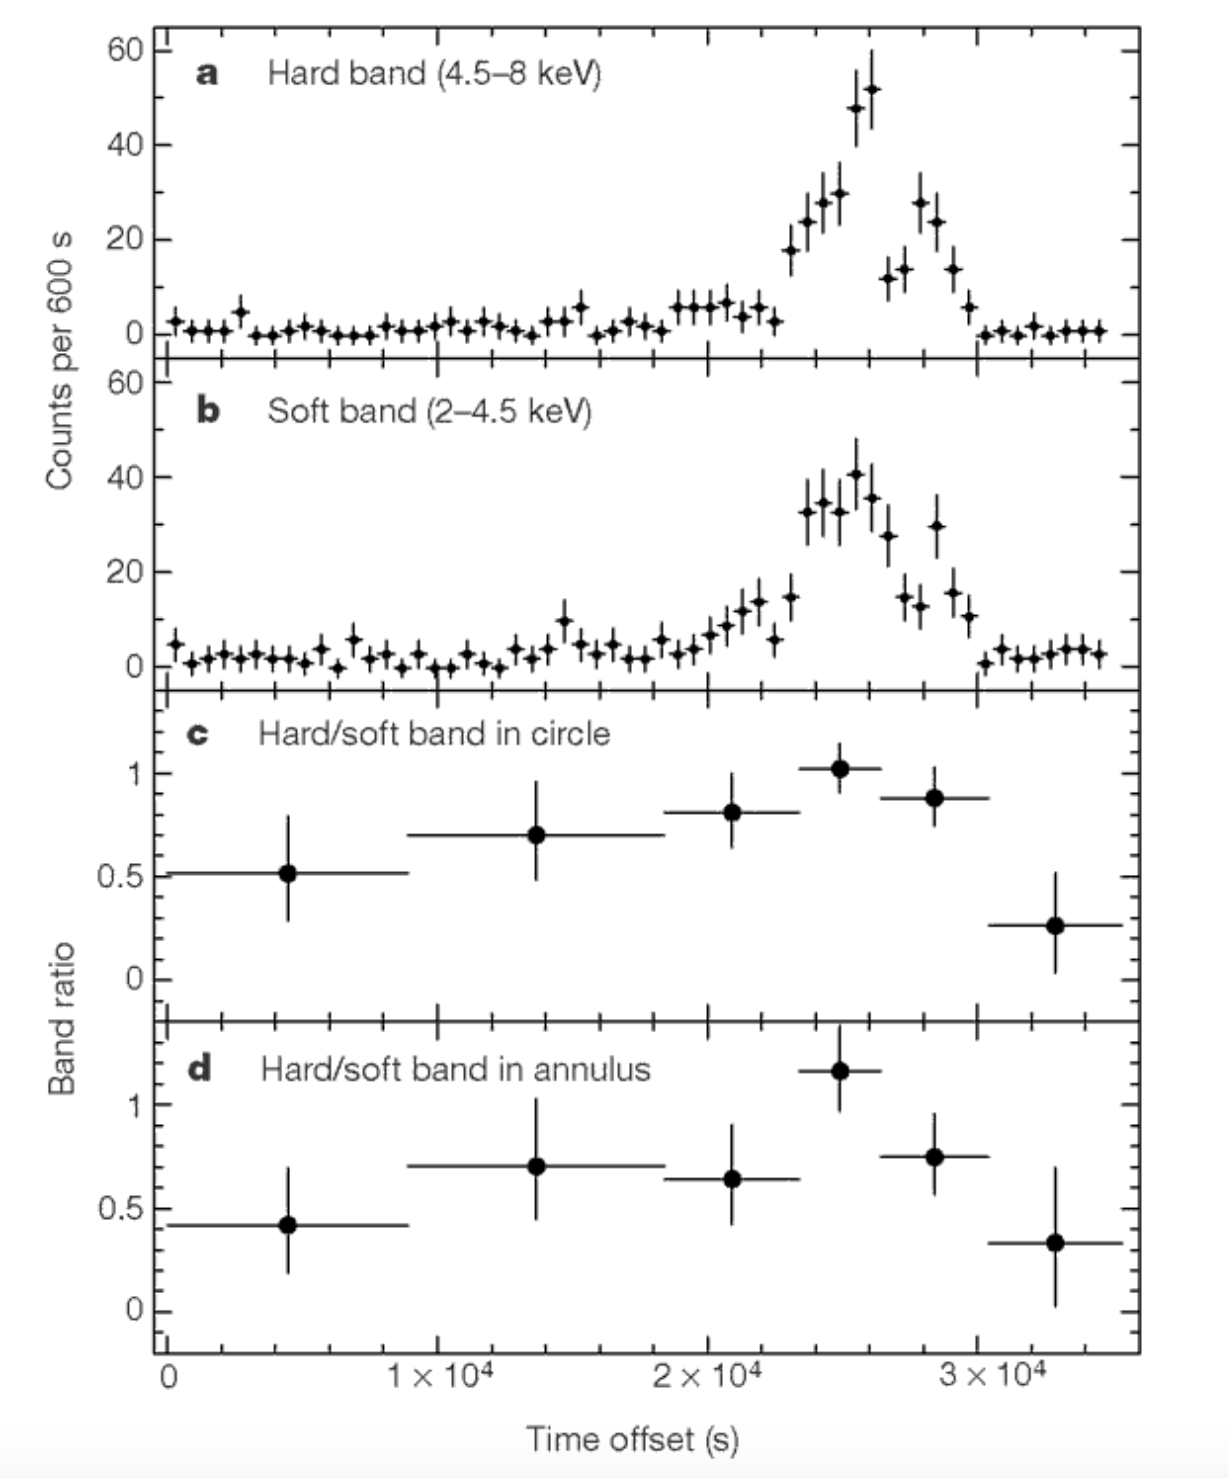
\includegraphics[width=0.7\textwidth]{galactic-center/sag-a-light-curve.png}
			\caption{Sag A* light curve, showing significant flaring on the timescale of a day.
				(from \url{https://heasarc.gsfc.nasa.gov/docs/objects/galaxies/sag-a star.html})}\label{gc:fig:light-curve}
		\end{figure}
	\end{enumerate}
\end{enumerate}

\section{Individual Homework}

Now that we have determined that Sag A* is an extremely dense, massive object --- but not quite certainly a black hole --- we are left to make plausibility arguments that allow us to
eliminate all other possible forms of matter. For each category of astrophysical objects listed
below, estimate the observational signatures of a hypothetical object with the mass you’ve
measured for Sag A*. Decide whether or not the estimated observable properties can be used
to rule out this alternative to a black hole.
\begin{enumerate}
	\item Main-Sequence Star/Cluster (Hint: the luminosity of massive stars scales as $M^4$, so
	what luminosity would a Sag A*-star have? What would be the luminosity of a cluster
	of sun-like stars with a total mass equal to that of Sag A*?)
	
	\item Brown Dwarf Star Cluster (Hint: A typical brown dwarf luminosity is $\sim 10^{-4} L_\textrm{\astrosun}$ and
	the maximum brown dwarf mass is $0.08M_\textrm{\astrosun}$. Brown dwarfs more massive than this are
	just stars, which you presumably ruled out above.)
	
	\item White Dwarf Star Cluster (Hint: a typical White Dwarf luminosity is $0.03L_\textrm{\astrosun}$, and the
	maximum white dwarf mass is $1.4M_\textrm{\astrosun}$. There are fundamental physical arguments that
	preclude the stable existence of a white dwarf above this mass.)
	
	\item Neutron Star Star Cluster (Hint: a typical Neutron Star luminosity is $10^{-6} L_\textrm{\astrosun}$ , and the
	maximum neutron star mass is estimated to be $1.4M_\textrm{\astrosun}$. This maximum mass is also
	derived from fundamental physics considerations). Would such a configuration, even if
	hypothetically possible, be physically reasonable?
\end{enumerate}